% Chapter 4

\chapter{Offloading de Cómputo} % Main chapter title

\label{ch:Chapter3} % For referencing the chapter elsewhere, use \ref{Chapter1} 

\lhead{Capítulo 3. \emph{Offloading de Cómputo}} % This is for the header on each page - perhaps a shortened title

En los últimos años, los usuarios de dispositivos móviles han sido testigos de un crecimiento considerable de aplicaciones
que son útiles en diferentes áreas: salud, entretenimiento, educación, entre otras. Dichas aplicaciones están disponibles 
(en algunos casos de manera gratuita) en distintas tiendas virtuales como (\emph{Google Play Store} \footnote{\url{https://play.google.com/store}
, último acceso en junio 2015}
, \emph{App Store} \footnote{\url{https://itunes.apple.com/us/genre/ios/id36}, último acceso en junio 2015}
y/o \emph{Amazon App Store} \footnote{\url{http://www.amazon.com/mobile-apps/b?node=2350149011}, último acceso en junio 2015}, entre otras. El crecimiento del mercado de programas móviles según
\emph{Transparency Market Research} ~\cite{transparencymarketresearch2014} (empresa que realiza investigación de mercado electrónico) 
pronostica que el mercado móvil crecerá rápidamente en los próximos cinco años, aumentando su valor en aproximadamente US\$ 16.97 billones
en el año 2014 a una valuación total de US\$ 54.89  billones en el año 2020. 

\begin{comment}
Hoy en día los dispositivos móviles ofrecen a los usuarios más aplicaciones, más y mejor ancho de banda para comunicarse y
más poder de procesamiento, 
los cuales colocan una carga pesada sobre el consumo de energía, mientras que los avances en la capacidad de batería crece en menor proporción
que los requerimientos en software de los usuarios modernos.

Se ha redescubierto que el offloading de computación usando  recursos no móviles disponibles a través de los canales de comunicación puede ayudar 
a reducir y conservar el consumo de energía \cite{5445167}, además que el offloading de aplicaciones puede resultar en tiempos de respuesta más 
rápidos, dado que los recursos remotos poseen mejores recursos de cálculo y almacenamiento que los dispositivos móviles. Este modelo es diferente
a las tradicionales arquitecturas cliente-servidor, en donde un cliente siempre migra el cálculo al servidor. El offloading de computo es diferente
del mismo modo a los modelos de migración usados en los sistemas multiprocesador y computación en grilla, donde un proceso puede ser migrado
para balancear la carga \cite{Powell:CSD-83-132}. La diferencia principal es que el \textit{offloading} migra procesos a servidores fuera del
entorno de computación inmediato al usuario, mientras que en computación en grilla ocurre de una computadora a otra con el mismo entorno 
computacional \cite{raey}.
\end{comment}

El uso intensivo y en conjunto de tales aplicaciones demandan una cantidad importante de procesamiento y de energía, los cuales 
no son abastecidos, esto por las limitaciones en los móviles ~\cite{6157576} : (i) baja capacidad de procesamiento, (ii) memoria limitada,
(iii) conexiones de red inestables, y (iv) duración de la batería limitada; debido a su naturaleza portátil. 

A pesar del gran avance tecnológico en hardware resaltado por la ley de Moore, el recurso más crítico en los dispositivos móviles 
es la densidad de la energía de las baterías, el cual ha tenido una tendencia de mejora considerablemente baja respecto a los demás 
componentes en la computación móvil \cite{1401839}. Tales limitaciones reducen la calidad del servicio 
que los usuarios móviles esperan tener.

La Computación en Nube para móviles (\textit{Mobile Cloud Computing}, MCC) tiene entre sus principales objetivos solucionar tales
inconvenientes proponiendo técnicas y \emph{frameworks} de \emph{offloading} al integrar los recursos en nube al entorno móvil de una
forma elástica y bajo demanda, no solamente para los dispositivos de gama baja sino para cualquier móvil que lo requiera \cite{6553297}. 

En ese escenario, a pesar de que es un área emergente de investigación, la industria móvil ya se ha beneficiado, por ejemplo: 
\begin{itemize}
\item El caso de la aplicación \emph{DeepFace}: El algoritmo de reconocimiento de rostros de \emph{Facebook} que alcanza una precisión del 97.35\%~\cite{taigman2014deepface}; 
\item La aplicación \emph{Google Now} \footnote{\url{http://www.google.com/landing/now/},  último acceso 
en febrero 2015} o \emph{Siri} \footnote{\url{http://www.apple.com/ios/siri/?cid=oas-us}, último acceso 
en febrero 2015 }: Son aplicaciones móviles para Android \footnote{\url{http://developer.android.com/index.html}, último acceso 
en febrero 2015} y iOS \footnote{\url{https://www.apple.com/ios/}, último acceso 
en febrero 2015} respectivamente, que utilizan algoritmos de 
reconocimiento de voz bajo una arquitectura basada en servicios (\textit{Service Oriented Arqchitecture}, SOA).
\item \emph{Dropbox} \footnote{\url{https://www.dropbox.com/}, último acceso en enero 2015},
el  cual permite extender la memoria secundaria del dispositivo en la nube otorgando seguridad de la información en caso de pérdida o robo del dispositivo móvil que lo utiliza, así como también sincronización con los dispositivos enlazados, entre otros beneficios. 
\end{itemize}

La técnica de \emph{Offloading} en el campo de MCC es utilizada para para aumentar virtualmente las capacidades del sistema móvil migrando 
partes de la aplicación a servidores en nube más potentes, de tal forma,  que mejore el tiempo de respuesta, el ahorro de energía y en muchos casos la precisión de los algoritmos. Dicha técnica se encuentra implementada en diferentes {\em frameworks}: MAUI~\cite{Cuervo:2010:MMS:1814433.1814441}, CloneCloud~\cite{chun2011clonecloud}, Cuckoo~\cite{kemp2012cuckoo}, 
COMET~\cite{gordon2012comet}, COFA~\cite{shivarudrappa2011cofa}.

La principal diferencia de estos {\em frameworks} con la arquitectura cliente-servidor es que el cálculo computacional puede o no ser enviado a ejecución remota. Esta decisión es provista por un algoritmo que considera parámetros variables: velocidad de ancho de banda, consumo de energía 
de la interfaz de red, tamaño de datos a enviar, entre otros. También existe una diferencia clave con el modelo \emph{grid computing} ya que las técnicas de \emph{offloading} migran los procesos
a un entorno de computación diferente al del usuario, en tanto que el modelo de \emph{grid} lo hace migrando a otro dentro del mismo entorno computacional. 

Se debe también tener en cuenta la naturaleza heterogénea, la cual es inherente a MCC presentando nuevos retos y desafíos en este nuevo campo de estudio. Debido al crecimiento competitivo de los compañías proveedoras, se generó heterogeneidad entre dispositivos móviles, plataformas de computación en nube y redes inalámbricas, dificultando principalmente la interoperabilidad y portabilidad~\cite{sanaei2014heterogeneity}.

%%%%%%%%%%%%%%%%%%%%%%%%%%%% OFFLOADING %%%%%%%%%%%%%%%%%%%%%%%%%%%%%%
\section{Offloading}
\label{offloading}
El término \emph{offloading} o \emph{cyber-foraging} fue introducido por Satyanarayanan \cite{943998} \emph {``Cyber-foraging es una forma efectiva de lidiar 
con este problema. La idea es aumentar dinámicamente los recursos computacionales de una computadora con conexión inalámbrica aprovechando 
la infraestructura de hardware cableada. A medida que el cálculo es más barato y más abundante, es sensato ``gastar'' estos recursos 
para mejorar la experiencia de usuario ''}.Inicialmente, \emph{Cyber-foraging} propone el aprovechamiento de computadoras estáticas 
en estado inactivo de una red local para aumentar las capacidades de los móviles inalámbricos. Hoy en día, la mayor estabilidad de las redes 
inalámbricas 
permiten que estos conceptos se hayan expandido de igual forma al uso de la computación en la nube con el fin de aumentar las capacidades 
de los dispositivos, por tal motivo usamos los términos \emph{cyber-foraging} y \emph{offloading} indistintamente en el presente texto.

El \emph{offloading} de aplicativos tiene como objetivo incrementar las capacidades de los sistemas móviles (extender la duración de la batería 
y mejorar el rendimiento de las aplicaciones \cite{5445167}) integrando la Computación en nube en los móviles. 
Sin embargo, en la práctica no es tan sencillo ya que debido a la heterogeneidad en MCC existen muchos factores que influyen sobre 
si es más adecuado el uso de los servicios en nube sobre la ejecución local. Tales factores dependen del ancho de banda de las red,
la interfaz de red a usar (Wifi, 3G and 4G), las cantidades de datos a transferir a través de la red, velocidad del servidor, memoria 
disponible y carga en el servidor. En este apartado damos un panorama general acerca de la viabilidad del \textit{offloading}, 
considerando los beneficios principales: mejora de velocidad y ahorro de energía; además, 
son descritos algunos factores externos e internos que influyen en la toma de decisiones al momento de hacer \emph{offloading}.


\subsection{Viabilidad de \textit{offloading} }
\label{subsec:offloadingdecision}

Dado que el proceso de \textit{offloading} transfiere parte del cómputo a un recurso computacional externo. Esta transferencia
depende de muchos factores no estándares inherentes a MCC (ver Sección \ref{sec:factors}), por lo tanto 
se requiere saber si aplicar la técnica de \textit{offloading} es necesaria y se tiene que analizar qué cálculo se migrará. 
En esta sección describimos dos factores de decisión  para aplicar \textit{offloading} y sus bases que la fundamentan. 

\subsubsection{Mejora del rendimiento}

A medida que las aplicaciones consumen más recursos computacionales, el \emph{offloading} se presenta como una opción atractiva 
\cite{balan2006simplifying} . Por ejemplo, propongamos el caso en el que un módulo crítico de telemedicina \cite{ryu2012telemedicine}
necesita realizar pre-procesamiento de señales en tiempo real; si el procesador de dicho módulo es demasiado lento, el cálculo pesado
puede ser migrado a servidores más potentes para su procesamiento.

El siguiente proceso es basado en la
investigación de \textit{Kumar et al.} \cite{raey}, el cual se ignoran los tiempos de conexión a la red y se asume que el tamaño del
programa es despreciable, o puede ser descargado de otro sitio mediante una red de alta velocidad. 

Se define a $S_w$ como la velocidad del sistema móvil y $w$ como la cantidad de cálculo a realizar de una parte $P$ que \textit{puede} ser 
migrada a la nube (no incluye funciones nativas, funciones que usen sensores, o funciones que administren dispositivos de entrada y/o salida).
Entonces, el tiempo de ejecución de la parte $P$ es : 

\begin{equation} \label{eq:mobilepartpartexecutiontime}
 \frac{w}{S_m}
\end{equation}

Si la parte $P$ es llevada a un servidor, enviar los datos de entrada $d_i$ toma $\frac{d_i}{B}$ segundos a un ancho de banda $B$. En esta 
sección el proceso de \textit{offloading} puede mejorar el rendimiento de la aplicación, incluyendo al 
cálculo y transmisión, puede ser realizado más rápido en el servidor. Ahora supongamos que $S_s$ sea la velocidad del servidor. Tiempo 
necesario para \textit{offload} al servidor y ejecutar la parte $P$ es: 

\begin{equation} \label{eq:serverpartexecutiontime}
 \frac{d_i}{B} + \frac{w}{S_s}  
\end{equation}

Entonces el proceso de \textit{offloading} mejora el rendimiento cuando la ecuación \ref{eq:mobilepartpartexecutiontime} es mayor que la ecuación
\ref{eq:serverpartexecutiontime}

\begin{equation} \label{eq:executiontimeFinal}
 \frac{w}{S_m}  > \frac{d_i}{B} +  \frac{w}{S_s} \Rightarrow w \left(\frac{1}{S_m} - \frac{1}{S_s} \right) > \frac{d_i}{B}.
\end{equation}

Esta desigualdad sostiene que:

\begin{itemize}
 \item Para un valor alto de $w$: El programa requiere computación pesada
 \item Para un valor alto de $S_s$: El servidor es más rápido.
 \item Para un valor pequeño de $d_i$: Una cantidad pequeña de datos es intercambiada.
 \item Para un valor alto de $B$: El ancho de banda es alto. 
\end{itemize}

La desigualdad muestra efectos limitados de la velocidad del servidor. Si se cumple que $\frac{w}{S_m}<\frac{d_i}{B}$, incluso si la
velocidad del servidor es infinitamente rápida (p. ej. $S_s \rightarrow \infty $  ), el proceso de \textit{offloading} no puede mejorar 
el rendimiento. Por lo que, solo tareas que requieren un cálculo pesado (un valor alto en $w$) con un intercambio ligero de datos (valor 
pequeño de $d_i$) deben ser consideradas. 


\subsubsection{Conservación de la energía}

La energía es la limitante de los sistemas móviles. Actualmente, los celulares ya no son usados solamente realizar llamadas; sino que también 
son usados para navegar
por internet, realizar video-llamadas, reproducir vídeos, procesamiento de \textit{streaming} de música, ejecución de juegos, entre otros.
Como resultado de 
la ejecución de todas esas aplicaciones el consumo de energía aumenta y por consecuencia se acorta la duración de la batería. La técnica de 
\textit{Offloading} tiene como objetivo conservar este recurso, enviando ejecuciones de tareas que demanden gran cantidad de 
procesamiento de la aplicación
a servidores remotos. 

El siguiente análisis propuesto por \textit{Kumar et al.}  \cite{raey} explica cuando las condiciones de las técnicas de \textit{offloading} 
conservan energía. Se define  
$p_m$ como la alimentación energética en el sistema móvil. Entonces, la energía del dispositivo móvil es para realizar una tarea puede 
ser obtenida modificando la ecuación 
\ref{eq:mobilepartpartexecutiontime}:

\begin{equation} \label{eq:energytoperform}
 p_m \times \frac{w}{s_m} 
\end{equation}

Sea $p_c$ la energía necesaria para enviar los datos desde un sistema móvil sobre la red. Por lo tanto, luego de enviar los datos, el sistema
necesita obtener la interfaz de red, mientras se espera los resultados. En este tiempo muerto, la energía consumida es $p_i$. Incorporando 
estos parámetros en la Ecuación \ref{eq:serverpartexecutiontime}, se tiene:

\begin{equation} \label{eq:energytoperform2}
 p_c \times \frac{d_i}{B} + p_i \times \frac{w}{S_s}
\end{equation}

Por lo tanto se puede inferir que el proceso de \textit{offloading} conserva energía cuando la Ecuación \ref{eq:energytoperform} es mayor que la Ecuación
\ref{eq:energytoperform2}. 

\begin{equation} % \label{eq:energytoperform3}
 p_m \times \frac{w}{s_m} > p_c \times \frac{d_i}{B} + p_i \times \frac{w}{s_s}
\end{equation}

\begin{equation} \label{eq:energyInequalityfinal}
 \Rightarrow w \times \left(\frac{p_m}{s_m} - \frac{p_i}{s_s} \right) > p_c \times \frac{d_i}{B}
\end{equation}

Se observa que las ecuaciones \ref{eq:executiontimeFinal} y \ref{eq:energyInequalityfinal} son muy similares. Para que el proceso de \textit{offloading}
conserve el energía, un cálculo pesado (un valor alto de $w$) y una ligera cantidad de datos (valor pequeño $d_i$) deben ser considerados. 

%floro

\subsection{Factores de decisión en \textit{offloading} }
%\subsection{Factores de decisión en \textit{offloading} }
\label{sec:factors}

En MCC, la heterogeneidad es consecuencia de la disputa de las grandes compañías por el mercado móvil. Esta competencia 
genera una variedad de servicios y/o productos singulares que en su mayoría no siguen un estándar, y por ende muchas veces se relega la
interoperabilidad y/o portabilidad \cite{sanaei2014heterogeneity}.


\textit{Sanae et al.} \cite{sanaei2014heterogeneity} identificó y clasificó la heterogeneidad presente en MCC, el cual lo representó en 
la Figura \ref{fig:heterogeinityRootsmcc}. Esta taxonomía presenta tres componentes (dispositivos móviles, la nube y las redes inalámbrica) 
que poseen raíces de heterogeneidad a nivel de : hardware, plataforma, características, interfaces de programación de aplicaciones (API,
\textit{Application Programming Interface}) y Red. Esta diversidad dificulta la toma de decisiones de los diferentes \emph{frameworks} 
de \emph{offloading}. Por ejemplo si consideramos dos celulares con arquitecturas distintas es probable uno de ellos tenga un
mejor tiempo de respuesta y la decisión más factible sea no aplicar la técnica de \emph{offloading}. Por lo tanto, la aplicación es 
probable que se ejecute localmente.
Similarmente, ocurre lo mismo en las entorno de las redes inalámbricas y en las características de la plataforma, lo cual  se profundizará en esta sección.

Considerando las raíces de la heterogeneidad en MCC, clasificamos los factores de decisión en \textit{offloading}
en tres grupos: características del dispositivo móvil, características de la aplicación
y características de red. Las cuales las presentamos a continuación: 

\subsubsection{Características del dispositivo móvil}
 La mayoría de dispositivos móviles están basados en computadoras con un conjunto de instrucciones
 reducidas (RISC, Reduced Instruction Set Computer) de 32 bits; sin embargo, existe una considerable variación en términos de velocidad
 del procesador,
 número de núcleos, cantidad de caché del procesador. Igualmente, existe una variedad importante entre los recursos del dispositivo móvil como
 la memoria memoria interna, fiabilidad de la antena inalámbrica y la capacidad de la batería. Tales parámetros necesitan ser contemplados 
 al momento de aplicar \emph{offloading}. En un futuro cercano con la entrada de la serie de procesadores ARM de 64 bits, entre los ya 
 tradicionales Cortex, se generará una heterogeneidad aún mas desafiante \footnote{\tiny \url{http://arm.com/about/newsroom/arm-discloses-technical-details-of-the-next-version-of-the-arm-architecture.php},
 último acceso en junio 2015}.
 
 Uno de los principales objetivos de proceso de \emph{offloading} es el ahorro de energía. Es por eso que considerar la precisión del gasto
 energético  individual de cada componente en tiempo real es un reto abierto.  
 
 \subsubsection{Características de la aplicación}
 
 Una métrica efectiva para decidir el proceso de \emph{offloading} es sobre las tareas que consumen alta carga computacional.
 No obstante, existen 
 algunas partes que no son convenientes para transferir. Porciones de código que ejecutan servicios locales como las interfaces de usuario o
 códigos que interactúan con componentes de entrada y/o salida como los sensores \cite{Cuervo:2010:MMS:1814433.1814441}, 
 métodos nativos del lenguaje de programación ya que pueden tener diferentes implementaciones en diferentes sistemas
 operativos \cite{gu2004adaptive} \cite{gordon2012comet} y tareas que necesitan recursos locales para ejecutarse
 \cite{Othman:1998:PCS:584007.584011}. 

\subsubsection{Características de red} 
 
 Debido al desplazamiento continuo del usuario, el dispositivo móvil necesita una red inalámbrica para iniciar la transferencia de cómputo a los 
 recursos computacionales en nube. Las redes inalámbricas del tipo Wi-Fi, 3G, 4G y WiMax son las más adecuadas, aunque tenemos que 
 considerar que cada una de estas interfaces consume una cantidad diferente de energía. Por ejemplo, como se observa en 
 la Figura \ref{fig:energyConsumption}, las redes 3G consumen más energía que las 
 redes Wi-FI con una reducida tasa de transferencia de bits, sin embargo ocurre lo contrario con una tasa alta
 de transferencia
 \cite{miettinen2010energy}. 
 
 \begin{figure}
   \centering
 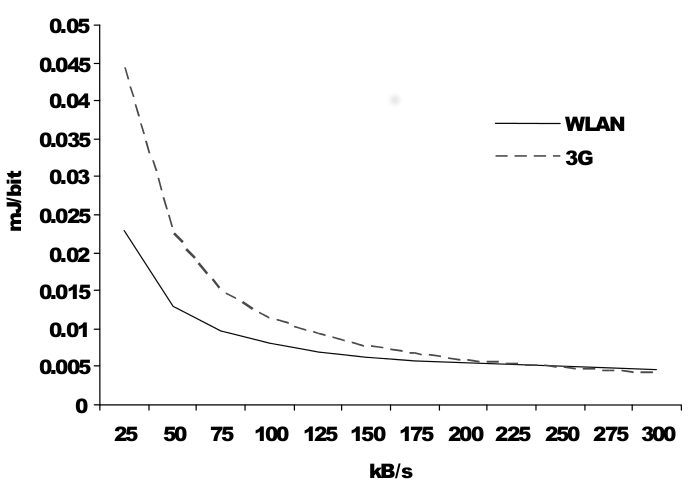
\includegraphics[scale=0.35]{Figures/energyConsumption.png}
 \caption{Consumo de energía por Bit de transferencia. WLAN vs 3G. Experimento realizado en celular Nokia N900 \cite{miettinen2010energy}}
 \label{fig:energyConsumption}
 \end{figure}

 
 Similarmente, una demora cuantiosa debido al ancho de banda de una red inalámbrica puede ser causante de un consumo de energía más alto, ya
 que la aplicación  se encuentra en estado inactivo a la espera del resultado.
 
 %%%%%%%%%%%%%%%%%%%%%%%%%%% OFFLOADING ALGORITHM %%%%%%%%%%%%%%%%%%%%%%%%%%%%%%%%%%%%5
 %%%%%%%%%%%%%%%%%%%%%%%%%%%%%%%%%%%%%%%%%%%%%%%%%%%%%%%%%%%%%%%%%%%%%%%%%%%%%%%%%%%%%%%%%%%%%%%%%%%%%%%%%%%%
 \section{Algoritmo de offloading }
\label{sec:offloadingAlgorithm}

En esta sección se presenta un algoritmo básico para la aplicación de \emph{offloading} de aplicaciones, el cual es representado 
en la Figura \ref{fig:offloadingAlgorithm}. Se debe resaltar que el algoritmo mostrado a continuación no es necesariamente  aplicado
en todos sistemas de \emph{offloading}.
El flujo comienza con la ejecución de la aplicación seguido por la revisión de los permisos del usuario para realizar \emph{offloading}. En caso posea estos privilegios, la aplicación revisa  si el servidor (sea 
de: red local o en la nube) está en conexión con el dispositivo móvil, revisando su conectividad. Posteriormente, se toma la decisión si realmente es viable y necesario el \emph{offloading}, cual sea el objetivo
principal: mejorar el rendimiento o ahorrar energía o ambos (descrito en la Sección
\ref{subsec:offloadingdecision}). Si la cuestión anterior es positiva, todo el entorno es favorable para su ejecución remota por lo que se migra el cálculo a servidores en la nube. En otro caso, la aplicación se ejecuta de manera local. 

El proceso \emph{offloading}, en especial la toma de decisión de \emph{offloading} es muy difícil de realizar con una adecuada precisión. 
Esto, debido a factores externos e internos del dispositivo móvil que fueron revisados en la Sección~\ref{sec:factors}.


 \begin{figure}[h]
   \centering
 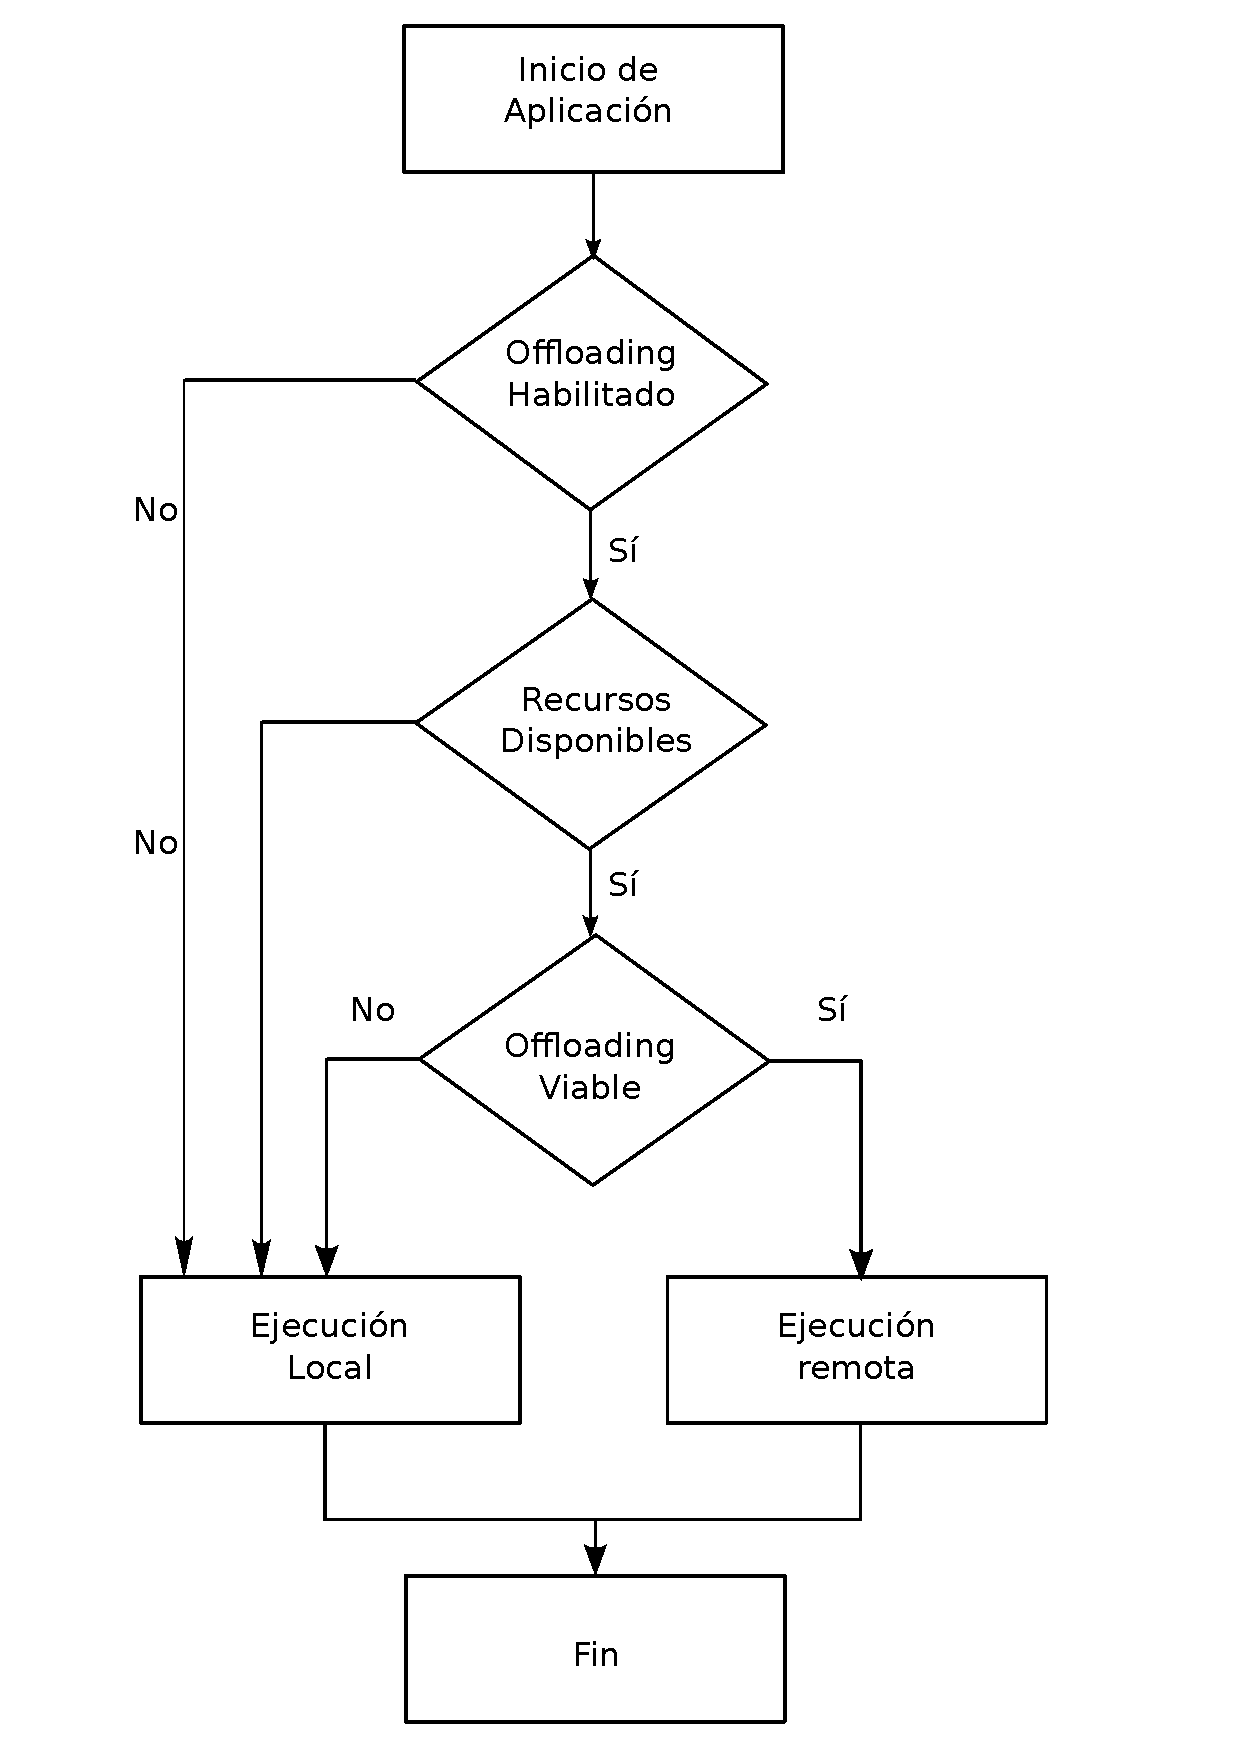
\includegraphics[scale=0.37]{Figures/processoffloadingcomputing}
 \caption{Proceso general de \emph{offloading}. Figura Adaptada de \cite{6553297} }
 \label{fig:offloadingAlgorithm}
 \end{figure}
 
 
 \section{Criterios para la clasificación de Offloading}
  \label{sec:metrics}
En las secciones anteriores fueron descritos los objetivos de la técnica de \emph{offloading} así como los factores que influyen en la toma de decisión para que ésta se realice. En este sección se describen los criterios de clasificación: tipo de \emph{offloading}, particionado de la aplicación y plataforma de despliegue. Posteriormente, se muestra una clasificación de los más importantes y actuales \emph{frameworks} de \emph{offloading} disponibles en MCC, la Tabla~\ref{table1:chart} muestra dicha clasificación siguendo los criterios anteriormente comentados.
 \begin{sidewaystable}
   %\begin{table*}[t]
 \footnotesize
 \caption{Algunas soluciones para el offloading de aplicaciones móviles}
 \begin{tabular}{lllllll}
\multicolumn{1}{c}{\cellcolor[HTML]{EFEFEF}{\color[HTML]{333333} \textbf{Año}}} & \multicolumn{1}{c}{\cellcolor[HTML]{EFEFEF}{\color[HTML]{333333} \textbf{Framework}}} & \multicolumn{1}{c}{\cellcolor[HTML]{EFEFEF}{\color[HTML]{333333} \textbf{Arquitectura}}} & \multicolumn{1}{c}{\cellcolor[HTML]{EFEFEF}{\color[HTML]{333333} \textbf{Objetivo Principal}}}            & \multicolumn{1}{c}{\cellcolor[HTML]{EFEFEF}{\color[HTML]{333333} \textbf{Tipo de Offloading}}} & \multicolumn{1}{c}{\cellcolor[HTML]{EFEFEF}{\color[HTML]{333333} \textbf{\begin{tabular}[c]{@{}c@{}}Plataforma \\ Cliente/Servidor\end{tabular}}}} & \multicolumn{1}{c}{\cellcolor[HTML]{EFEFEF}{\color[HTML]{333333} \textbf{\begin{tabular}[c]{@{}c@{}}Campo de \\ Aplicación\end{tabular}}}} \\
2002                                                                            & Spectra \cite{flinn2002balancing}                                                         & Orientado a Servicios                                                                    & \begin{tabular}[c]{@{}l@{}}Ahorro de Energía y reducción \\ de tiempo de Ejecución\end{tabular} & Estático                                                                                       & \begin{tabular}[c]{@{}l@{}}Entorno \\ Simulado\end{tabular}                                                                                        & \begin{tabular}[c]{@{}l@{}}Procesamiento\\ de Audio y \\ Documentos\end{tabular}                                     \\
2003                                                                            & Chroma \cite{balan2003tactics}                                                               & Orientado a Servicios                                                                    & Reducción de tiempo de Ejecución                                                                & Estático                                                                                       & \begin{tabular}[c]{@{}l@{}}Entorno\\ Simulado\end{tabular}                                                                                         & \begin{tabular}[c]{@{}l@{}}Procesamiento\\ de Imágenes\end{tabular}                                                  \\
2010                                                                            & MAUI \cite{Cuervo:2010:MMS:1814433.1814441}                                                  & Virtualización                                                                           & \begin{tabular}[c]{@{}l@{}}Ahorro de Energía \end{tabular}                    & Dinámico                                                                                       & \begin{tabular}[c]{@{}l@{}}Windows \\ Mobile / .Net\end{tabular}                                                                                   & \begin{tabular}[c]{@{}l@{}}Procesamiento\\ de Imágenes /\\ Juegos\end{tabular}                                       \\
2011                                                                            & CloneCloud \cite{chun2011clonecloud}                                                         & Virtualización                                                                           & \begin{tabular}[c]{@{}l@{}}Ahorro de Energía y reducción \\ de tiempo de Ejecución\end{tabular} & Dinámico                                                                                       & Android/Dalvik                                                                                                                                     & \begin{tabular}[c]{@{}l@{}}Análisis de Virus\\ /Búsqueda de \\ imágenes\end{tabular}                                 \\
2011                                                                            & COFA \cite{shivarudrappa2011cofa}                                                            & Orientado a Servicios                                                                    & \begin{tabular}[c]{@{}l@{}}Ahorro de Energía y reducción \\ de tiempo de Ejecución\end{tabular} & Estático                                                                                       & Android/Dalvik                                                                                                                                     & \begin{tabular}[c]{@{}l@{}}Cálculos\\  matemáticos\end{tabular}                                                      \\
2012                                                                            & COMET \cite{gordon2012comet}                                                                & Virtualización                                                                           & \begin{tabular}[c]{@{}l@{}}Reducción de tiempo de Ejecución \end{tabular}       & Dinámico                                                                                       & \begin{tabular}[c]{@{}l@{}}CyanogenMod\\ (Android)/Dalvik\end{tabular}                                                                             & \begin{tabular}[c]{@{}l@{}}Aplicaciones \\ Web\end{tabular}                                                          \\
2012                                                                            & Cuckoo \cite{kemp2012cuckoo}                                                                 & Orientado a Servicios                                                                    & \begin{tabular}[c]{@{}l@{}}Ahorro de Energía y reducción \\ de tiempo de Ejecución\end{tabular} & Estático                                                                                       & Android/JavaVM                                                                                                                                     & \begin{tabular}[c]{@{}l@{}}Juegos / \\ Procesamiento \\ de Imágenes\end{tabular}                                    
\end{tabular}
\label{table1:chart}
%\end{table*}
 \end{sidewaystable}
 \subsection{Particionado de la Aplicación}
 La presente investigación se basa principalmente en dos tipos de arquitecturas al momento de realizar el particionado:
 ``arquitecturas basadas en servicios'' y ``virtualización'' \cite{fernando2013mobile}.
 El primero es realizado entre el dispositivo móvil y el servidor vía protocolos como por ejemplo: llamadas a procedimiento remoto 
 (RPC, Remote Procedure Call), invocación de métodos remotos(RMI, Remote Method Invocation) y sockets.
 Dos ejemplos que utilizan estos protocolos son los \emph{frameworks} Chroma~\cite{balan2003tactics} y Spectra~\cite{flinn2002balancing}
 los cuales poseen pre-instalado en sus servidores servicios RPC para el proceso de \emph{offloading}. Otro ejemplo es el {\em framework 
 Cuckoo} ~\cite{kemp2012cuckoo}, \textit{framework} para
 \emph{offloading}  basado en Android OS\footnote{\url{http://developer.android.com/index.html}, último acceso en setiembre 2015}, como se observa en su arquitectura de la Figura ~\ref{fig:cuckoo}, utiliza interfaces
 para la comunicación con componentes
 nativos siguiendo el modelo {\em stub/proxy} en el lenguaje de programación Java. El {\em framework Cuckoo} utiliza el modelo por defecto 
 de Android {\em activity/service} que separa las actividades (métodos de interacción con el usuario) de los servicios
 (métodos de cómputo pesado).
 
\begin{figure}
\centering
  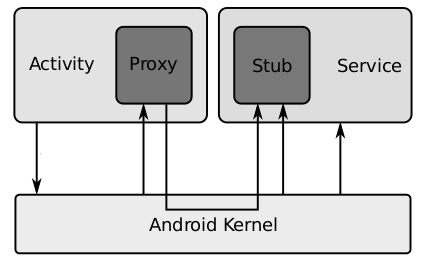
\includegraphics[scale=0.5]{Figures/cuckoo.png}
  \caption{Arquitectura del \emph{framework} Cuckoo \cite{kemp2012cuckoo}}
  \label{fig:cuckoo}
\end{figure}

 En el segundo tipo arquitectural, la virtualización, consiste en transferir la imagen de la memoria 
 de una máquina virtual (VM, \textit{Virtual Machine}) desde un servidor origen a un servidor destino sin detener su ejecución~\cite{clark2005live}. Durante la migración las páginas de memoria de la MV son copiadas previamente sin generar interrupción alguna en el sistema operativo, de tal modo que da la sensación de una migración natural. Una ventaja es que el código de la aplicación no necesita ser rescrito y provee una alta y segura ejecución, debido a que los límites de la MV lo aíslan. MAUI~\cite{Cuervo:2010:MMS:1814433.1814441} es \emph{framework} el cual usa una una mezcla de migración, entre MV y partición de código. Las aplicaciones que usan MAUI pueden transferir calculos a servidores tanto locales como remotos que estén sobre la infraestructura en la plataforma {\bf .NET}. Otro ejemplo es el \emph{framework} CloneCloud \cite{chun2011clonecloud} el cual usa migración de MV para transferir parte de la carga de la aplicación a servidores.
 
\subsection{Tipos de Offloading}

A fin de adaptar técnicas de \textit{offloading} en una aplicación, es concerniente al desarrollador conocer las posibles maneras para implementar,
así como sus posibles ventajas y desventajas. Tal adaptación puede ocurrir de dos maneras: de forma estática o dinámica~\cite{murarasu2009mobile}. En el primer enfoque el desarrollador define que
 secciones de código se ejecutarán remotamente. Esto ocurre en la fase de diseño o en la instalación y por 
 lo tanto cuando se inicia el ejecutable, el \emph{framework} conoce de antemano que partes del programa pueden ser
 enviados a ejecución remota. La 
 principal ventaja es que no existe una prominente sobrecarga en la aplicación, por tal motivo en este enfoque es necesario que los factores 
 que influyen en el algoritmo de decisión ( que describimos en la sección \ref{sec:factors}) sean predichos lo más exacto posible. Parámetros como
 poder de cálculo o ancho de banda en el lado del servidor son valores muy estables debido a que los grandes proveedores garantizan un nivel mínimo de 
 rendimiento.
 Algunos algoritmos de predicción de estos factores son: predicción basada en los registros históricos \cite{gurun2004nwslite} y predicción
 probabilística \cite{rong2003extending}. 
 Por otro lado, en el enfoque dinámico la ubicación de la parte a transferir no esta predeterminado por el desarrollador y tiene que 
 ser calculado generalmente en tiempo de ejecución, lo cual genera sobrecarga de cómputo. En este enfoque de igual manera existen mecanismos 
 de predicción para la toma de decisiones.Por ejemplo algunas propuestas construyen modelos de Markov como un modelo de movilidad (basados en
 el histórico de conexiones a puntos de acceso Wi-Fi), entonces es entrenado con patrones de movilidad del usuario \cite{lee2013user}. 
 En cambio, Wolski \cite{wolski2008using} en su investigación propone que el ancho de banda sea predicha usando un esquema bayesiano.
 

 \subsection{Plataforma de despliegue}
 
 Las soluciones para el \emph{offloading} de aplicaciones requieren desplegarse en plataformas móviles y en plataformas en nube. Para este motivo
 existe una pluralidad de plataformas heterogéneas en la computación en nube y en la computación móvil . 
 Esta heterogeneidad (como se observó en la Figura \ref{fig:heterogeinityRootsmcc} ) generalmente limita a los sistemas de
 \emph{offloading} a ejecutarse en todas las plataformas. Tal es el caso de 
 CloneCloud \cite{chun2011clonecloud} que explota el sistema operativo de código abierto AndroidOS
 para integrar su solución. Este sistema despliega una versión modificada de la máquina virtual de Dalvik (MV del sistema 
 Operativo Android) \cite{ehringer2010dalvik} en un servidor en la Nube con el fin de que acepte la transferencia de la aplicación.
 
 Otro ejemplo es el caso de MAUI \cite{Cuervo:2010:MMS:1814433.1814441}, el cual implementa una arquitectura basada en \emph{Windows Mobile}
 \footnote{\url{https://www.windowsphone.com/en-us}, último acceso en enero 2015}
 para su implementación  en el móvil, entre tanto que en el servidor  se despliega en un arquitectura \emph{.NET}. Cuckoo \cite{kemp2012cuckoo}
 por el lado del cliente está basado en Android, mientras que el servidor se ejecuta sobre la MV de Java. Este hecho hace posible que el 
 servidor de Cuckoo sea genérico y puede desplegarse sin mayor esfuerzo en cualquier tipo de servidor. En el caso de COMET \cite{gordon2012comet}
 en el lado del cliente se usa CyanogenMod \footnote{\url{http://www.cyanogenmod.org/}, último acceso en febrero 2015},
 una versión libre de Android mantenida por la Comunidad CyanogenMod.
 
 \subsection{Campo de Aplicación}
 
 Múltiples dominios pueden ser beneficiadas debido a la aplicación de \textit{offloading}. Para tal prueba del concepto, 
 los investigadores han 
 implementado aplicaciones sobre diferentes áreas. En esta sección presentamos ejemplos que demuestran el beneficio del empleo de 
 \textit{offloading}: 
 
 \begin{enumerate}
  \item Cálculos Matemáticos: Funciones matemáticas complejas, tal como la multiplicación de matrices de gran tamaño, o la 
  la secuencia de \textit{fibonacci} de un número considerable, esta última fue implementada por \textit{Shivarudrappa et al.} en su trabajo
  para aliviar carga computacional llamado COFA \cite{shivarudrappa2011cofa} 
  \item Procesamiento de Señales: Las tareas de procesamiento de señales como voz o imágenes demandan una alta carga computacional, y por ende 
  un consumo energético elevado. Por ejemplo, una aplicación de reconocimiento de patrones en imágenes como lo aplicaron los autores de MAUI 
  \cite{Cuervo:2010:MMS:1814433.1814441} en su caso de estudio, o en el caso de la aplicación \textit{eyeDentify}, la cual es 
  implementa usando el \textit{framework Cuckoo} \cite{kemp2012cuckoo} para el reconocimiento de objetos en imágenes. 
  \item Juegos: Las aplicaciones de juegos usualmente requieren un poder de cómputo pesado para mantener un renderizado suave de cada
  \textit{frame}, de tal manera
  que la interacción con el usuario sea rápida. En el trabajo propuesto por \textit{Kemp et al.} \cite{kemp2012cuckoo}, se presenta la aplicación
  \textit{PhotoShoot}, un juego multi-jugador de la categoría de disparos en primera persona (FPS, First Person Shooter) que sin la aplicación de 
  \textit{offloading}, a más lento el procesador del dispositivo móvil, más tiempo toma el disparo en ser analizado, lo cual da al usuario 
  con el móvil limitado una seria desventaja. Por ende, aplicar \textit{offloading} de cierto modo establece un juego más justo.
  \item Análisis de Virus: Estimando la creciente amenaza de virus y \textit{malwares}, las aplicaciones de la categoría antivirus están siendo
  una parte fundamental de los sistemas móviles. Sin embargo, el uso de dichos aplicativos demandan una gran cantidad de cálculo que consume
  una cantidad considerable de energía. El proceso de adaptar técnicas de \textit{offloading} en este dominio , podría aliviar estas limitaciones
  al realizar un escaneo 
  en la nube de una imagen del celular para ahorrar energía (asumiendo que el dispositivo móvil y su clon en la nube, están sincronizados). 
  Un ejemplo en esta área es el de \textit{CloneCloud} \cite{chun2011clonecloud}, el cual es usado para el caso de estudio de análisis de virus. 
  \cite{DBLP:journals/corr/abs-1105-3232}. 
  
 \end{enumerate}

 
  Similarmente, existe una variedad de aplicaciones que pueden tomar ventaja del uso de MCC. Sin embargo, aún existen aún retos abiertos consecuencia
  de su heterogeneidad presente.
 



























